%!TEX root=../master.tex
%========================================================================================================
% REGRESSION
%========================================================================================================
\section{Regression}
\subsection{Linear Regression}
Simple
$y_n \approx f(\mathbf{x_n}) := w_0 + w_1 x_{n1}$\newline
Multiple\newline
$f(\mathbf{x_n}) := w_0 + \sum_{j=1}^D w_j x_{nj} = \tilde{\mathbf{x}}_n^T \mathbf{w}$\newline
If $D > N$ the task is under-determined (more dimensions than data) $\rightarrow$ regularization.

\section{Cost functions}
MSE $= \frac{1}{N} \sum_{n=1}^N [y_n - f(\mathbf{x_n})]^2$ Not good with outliers.\newline
MAE $= \frac{1}{N} \sum_{n=1}^N |y_n - f(\mathbf{x_n})|$\newline
Error $e_n = y_n - f(\mathbf{x_n})$
\subsection{Convexity}
A line joining two points never intersects with the function anywhere else.
$f(\lambda \mathbf{u} + (1-\lambda)\mathbf{v}) \le \lambda f(\mathbf{u}) + (1-\lambda) f(\mathbf{v})$ with $\lambda \in [0;1]$.
A strictly convex function has a unique global minimum $w^*$. Sums of convex functions are convex.

A function must always lie above its linearisation: \newline $\mathcal{L}(u) \ge \mathcal{L}(w) + \nabla \mathcal{L}(w)^T (u-w) \forall u,w$.

A set is convex iff line segment between any two points of $\mathcal{C}$ lies in $\mathcal{C}$ : $\theta u + (1 - \theta) v \in \mathcal{C}$

%========================================================================================================
% OPTIM
%========================================================================================================
\section{Optimisation}
Find $\mathbf{w^*} \in \mathcal{R}^D$ which $min\,\,\mathcal{L}(\mathbf{w})$.\newline
Gradient $\nabla \mathcal{L} := \begin{bmatrix} \frac{\partial \mathcal{L}(\mathbf{w})}{\partial w_1} & \dots & \frac{\partial \mathcal{L}(\mathbf{w})}{\partial w_D} \end{bmatrix}$

\subsection{Gradient descent}

$\mathbf{w^{(t+1)}} = \mathbf{w^{(t)}} - \gamma \nabla \mathcal{L}(\mathbf{w^{(t)}})$. Very sensitive to ill-conditioning.

GD - Linear Reg

$\mathcal{L}(\mathbf{w}) = \frac{1}{2N} (\mathbf{y} - X\mathbf{w})^T(\mathbf{y} - X\mathbf{w}) \rightarrow$ \newline $ \nabla \mathcal{L}(\mathbf{w}) = - \frac{1}{N} X^T(\mathbf{y} - X\mathbf{w})$. Cost: \newline $O_{err} = 2ND + N$ and $O_{w} = 2ND + D$.

\subsection{SGD}

$\mathcal{L} = \frac{1}{N} \sum{\mathcal{L}}_n(\mathbf{w})$ with update $\mathbf{w}^{(t+1)} = \mathbf{w}^{(t)} - \gamma \nabla \mathcal{L}_n(\mathbf{w}^{(t)})$.

\subsection{Mini-batch SGD}

$\mathbf{g} = \frac{1}{|B|} \sum_{n\in B}{\nabla \mathcal{L}}_n(\mathbf{w}^{(t)})$ with update $\mathbf{w}^{(t+1)} = \mathbf{w}^{(t)} - \gamma \mathbf{g}$.

\subsection{Subgradient at $w$}

$\mathbf{g} \in \mathbb{R}^D$ such that $\mathcal{L}(u) \ge \mathcal{L}(w) + \mathbf{g}^T (u-w)$. Example subgradient for MAE: $h(e) = |e| \rightarrow g(e) = {sgn(e) \text{ if } e \ne 0, \lambda \text{ otherwise }}$. We get the gradient:\newline $\nabla \mathcal{L}_{MAE} = - \frac{1}{N} \sum_n sgn(x_n) \nabla f(x_n)$.

\subsection{Projected SGD}

$\mathbf{w}^{(t+1)} = \mathcal{P_C} [\mathbf{w}^{(t)} - \gamma \nabla \mathcal{L}(\mathbf{w}^{(t)})]$

\subsection{Newton's method}
Second order (more expensive $O(ND^2 + D^3)$ but faster convergence).

$w^{(t+1)} = w^{(t)} - \gamma^{(t)} (H^{(t)})^{-1} \nabla \mathcal{L}(w^{(t)})$


\subsection{Optimality conditions}
Necessary : $\nabla \mathcal{L} (\mathbf{w}^*) = 0$
Sufficient : Hessian PSD $\mathbf{H}(\mathbf{w}^*) := \frac{\partial^2 \mathcal{L}(\mathbf{w}^*)}{\partial w \partial w^T}$

%========================================================================================================
% LEAST SQUARES
%========================================================================================================

\section{Least Squares}
\subsection{Normal Equation}
$X^T (\mathbf{y} - X\mathbf{w})= 0 \Rightarrow$\newline$\mathbf{w^*} = (X^TX)^{-1}X^T\mathbf{y} \text{ and } \mathbf{\hat{y}_m} = \mathbf{x_m}^T \mathbf{w^*}$
Graham matrix invertible iff $rank(X) = D$ (use SVD $X = USV^T \in \mathbb{R}^{N\times D}$ if this is not the case to get pseudo-inverse $\mathbf{w^*} = V\tilde{S}U^T$ with $\tilde{S}$ pseudo-inverse of $S$).

\section{Likelihood}
Probabilistic model $y_n = \mathbf{x_n}^T\mathbf{w} + \epsilon_n$.
Probability of observing the data given a set of parameters and inputs :
$p(\mathbf{y}|X, \mathbf{w}) = \prod p(y_n|\mathbf{x_n}, \mathbf{w})  = \prod \mathcal{N} (y_n | \mathbf{x_n}^T\mathbf{w}, \sigma^2)$

Best model maximises log-likelihood $\mathcal{L}_{LL} = -\frac{1}{2\sigma^2} \sum(y_n-x_n^Tw)^2+cst$.


%========================================================================================================
% REGULARISATION
%========================================================================================================
\section{Regularization}
\subsection{Ridge Regression}
$\mathcal{L}(\mathbf{w}) = \frac{1}{2} (\mathbf{y} - X\mathbf{w})^T(\mathbf{y} - X\mathbf{w}) + \frac{\lambda}{2} ||\mathbf{w}||^2_2 \rightarrow$
$\mathbf{w^*_{ridge}} = (XX^T + \lambda I_D)^{-1}X^T\mathbf{y} = X^T(XX^T + \lambda I_N)^{-1}\mathbf{y}$

Can be considered a MAP estimator : $\mathbf{w^*_{ridge}} = arg min_w - log(p(w|X,y))$

\subsection{Lasso}
Sparse solution.
$\mathcal{L}(w) = \frac{1}{2N} (y - Xw)^T(y - Xw) + \lambda ||w||_1 $

%========================================================================================================
% MODEL SELECTION
%========================================================================================================
\section{Model Selection}
\subsection{Bias-Variance decomposition}
Small dimensions : large bias, small variance.
Large dimensions : small bias, large variance.
Error for the val set compared to the emp distr of the data goes down like $\frac{1}{\sqrt{|\text{validation points}|}}$ and goes up like $\sqrt{ln(|\text{hyper parameters}|)}$


%========================================================================================================
% CLASSIFICATION
%========================================================================================================
\section{Classification}
\subsection{Optimal}
$\hat{y}(\mathbf{x}) = argmax_{y\in \mathcal{Y}} p(y|\mathbf{x})$

\subsection{Logistic regression}
$\sigma(z) = \frac{e^z}{1+e^z}$ to limit the predicted values $y\in [0;1]$ ($p(1|\mathbf{x}) = \sigma(\mathbf{x}^T\mathbf{w})$ and $p(0|\mathbf{x}) = 1-\sigma(\mathbf{x}^T\mathbf{w})$). We decide with respect to 0.5

Likelihood

$p(y | X,w) = \prod p(y_n|x_n) = \prod_{n:y_n=0} p(y_n=0|x_n) ... \prod_{n:y_n=K} p(y_n=K|x_n) = \prod^K_k \prod^N_n [p(y_n = k | x_n,w)]^{\tilde{y}_{nk}}$ where ${tilde{y}_{nk}} = 1$ if $y_n=k$.

For binary classification

$p(y | X, w) = \prod p(y_n|x_n) = \prod_{n:y_n=0} p(y_n=0|x_n) \prod_{n:y_n=1} p(y_n=1|x_n) = \prod^N_n \sigma({x_n^T w})^{y_n}[1-\sigma({x_n^T w})]^{1-y_n}$

Loss

$\mathcal{L}(w) = \sum_{n=1}^N ln(1 + exp(x_n^T w)) - y_n x_n^T w$ which is convex in $w$.

Gradient

$\nabla \mathcal{L}(w) = \sum_{n=1}^N x_n (\sigma(x_n^T w) - y_n) = X^T[\sigma(Xw) - y]$ (no closed form solution).

Hessian

$H(w) = X^T S X$ with $S_{nn} = \sigma(x_n^T w)[1-\sigma(x_n^T w)]$

\subsection{Exponential family}
General form

$p(y|\eta) = h(y) exp[\eta^T \psi(y) - A(\eta)]$ where

Cumulant

$A(\eta) = ln[\int_y h(y) exp[\eta^T \psi(y)] dy]$
\newline
$\nabla A(\eta) = \mathbb{E}[\psi(y)] = g^{-1}(\eta)$
\newline
$\nabla^2 A(\eta) = \mathbb{E}[\psi\psi^T] - \mathbb{E}[\psi]\mathbb{E}[\psi^T]$

Link function

$\eta = g(\mu) \Leftrightarrow \mu = g^{-1}(\eta)$

$\eta_{gaussian} = (\mu / \sigma^2, - 1 / 2 \sigma^2)$
; $\eta_{poisson} = ln(\mu)$
; $\eta_{bernoulli} = ln(\mu / 1 - \mu)$
; $\eta_{general} = g^{-1}(\frac{1}{N} \sum_{n=1}^N \psi(y_n))$

$\nabla \mathcal{L}(w) X^T [g^{-1}(Xw)- \psi(y)]= 0$

\subsection{Nearest Neighbor Models}
Performs best in low dimensions.
\subsubsection{k-NN}
$f_{S^{t,k}}(x) = \frac{1}{k} \sum_{n:x_n\in ngbh_{S{t,k}(x)}} y_n$
Pick odd $k$ so there is a clear winner.
Large $k \rightarrow$ large bias small variance (inv.)

\subsubsection{Error bound}
$\mathbb{E}[\mathcal{L}_{St}] \le 2 \mathcal{L}_{f^*} + 4 c \sqrt{d} N^{-1/d+1}$

\subsection{Support Vector Machines (SVM)}
Logistic regression with hinge loss :
$min_w \sum_{n=1}^N [1-y_n x_n^T w]_+ + \frac{\lambda}{2} ||w||^2$ where $y \in [-1;1]$ is the label and $hinge(x)= max\{0,x\}$. Convex but not differentiable so need subgradient.

We can also use duality : $\mathcal{L}(w) = max_{\alpha} G(w, \alpha)$. For SVM
$min_{w} max_{\alpha \in [0,1]^N} \sum \alpha_n (1 - y_nx_n^Tw) + \frac{\lambda}{2} ||w||^2$ differentiable and convex.

Can switch $max$ and $min$ when convex in $w$ and concave in $\alpha$. This can make the formulation simpler:

$w(\alpha) = \frac{1}{\lambda} \sum \alpha_n y_n x_n = \frac{1}{\lambda} X^T diag(y) \alpha$ which yields the optimisation problem:
$max_{\alpha \in [0,1]^N} \alpha^T\mathbf{1} - \frac{1}{2\lambda} \alpha^T Y X X^T Y \alpha$
The solution is sparse ($\alpha_n$ is the slope of the lines that are lower bounds to the hingle loss).

\subsection{Kernel Ridge Regression}
From duality $w^* := X^T \alpha^*$ where $\alpha^* := (K + \lambda I_N)^{-1}y$ and $K=XX^T = \phi^T(x) \phi(x) = \kappa(x,x')$ (needs to be PSD and symmetric).


%========================================================================================================
% UNSUPERVISED LEARNING
%========================================================================================================
\section{Unsupervised Learning}
\subsection{K-means clustering}

$min \mathcal{L}(z,\mu) = \sum_n^N \sum_k^K z_{nk} ||x_n - \mu_k||^2_2$ with $z_{nk} \in \{0,1\}$ (unique assignments: $\sum_k z_{nk} = 1$).

Algorithm (Coordinate Descent)
\begin{enumerate}
\item $\forall n$ compute $z_n = \begin{cases}
	1 \text{ if } k = argmin_j || x_n - \mu_k||^2 \\
	0 \text{ otherwise }
   \end{cases}$
\item $\forall k$ compute $\mu_k = \frac{\sum_n z_{nk} x_n}{\sum_n z_{nk}}$
\end{enumerate}

Issues
\begin{enumerate}
	\item Heavy computation
	\item Spherical clusters
	\item Hard clusters
\end{enumerate}

Probabilistic model
$p(X|\mu,z) = \prod_n^N \mathcal{N}(x_n|\mu_k,I) = \prod_n^N \prod_k^K \mathcal{N}(x_n|\mu_k,I)^{z_{nk}}$

\subsection{Gaussian Mixture Models}
$p(X|\mu,z) = \prod_n^N p(x_n|z_n,\mu_k,\Sigma_k)p(z_n|\pi)
= \prod_n^N \prod_k^K [\mathcal{N}(x_n|\mu_k,\Sigma_k)]^{z_{nk}} \prod_k^K [\pi_k]^{z_{nk}}$ where $pi_k = p(z_n=k)$

Marginal likelihood: $z_n$ are latent variables so they can be factored out from the likelihood $p(x_n|\theta) = \sum \pi_k \mathcal{N}(x_n|\mu_k, \Sigma_k)$. (number of parameters reduced from $O(N)$ to $O(D^2K)$.

\subsection{EM}
\subsubsection{GMM}
Intialize $\mu^{(1)}, \Sigma^{(1)}, \pi^{(1)}$.
\begin{enumerate}
\item E-step: Compute the assignments. $q_{kn}^{(t)} := \frac{\pi_k^{(t)} \mathcal{N}(x_n|\mu_k^{(t)}, \Sigma_k^{(t)})}{ \sum_k^K \pi_k^{(t)} \mathcal{N}(x_n|\mu_k^{(t)}, \Sigma_k^{(t)}) }$
\item Compute Marginal Likelihood
\item M-step: Update

$\mu^{(t+1)} = \frac{\sum_n q_{kn}^{(t)} x_n}{\sum_n q_{kn}^{(t)}}$

$\Sigma^{(t+1)} = \frac{\sum_n q_{kn}^{(t)}(x_n - \mu^{(t+1)})(x_n - \mu^{(t+1)})^T}{\sum_n q_{kn}^{(t)}}$

$\pi^{(t+1)} = \frac{1}{N} \sum_n q_{kn}^{(t)}$
\end{enumerate}

\subsubsection{General}
$\theta^{(t+1)} := argmax_{\theta} \sum_n^N \mathbb{E}_{p(z_n|x_n,\theta^{(t)})}[log\,\, p(x_n,z_n|\theta)]$

%========================================================================================================
% Matrix Factorizations
%========================================================================================================
\section{Matrix Factorizations}
\subsection{Prediction}
Find $\mathbf{X} \approx \mathbf{W}\mathbf{Z}^T$ where $\mathbf{W} \in \mathbb{R}^{D\times K}$ and $\mathbf{Z} \in \mathbb{R}^{N\times K}$ with $K << D,N$. Large $K\rightarrow$ overfitting. If $K \ge max\{D,N\}$ trivial solution ($W=\mathbf{1}_D$ or $Z=\mathbf{1}_N$).

Quality of reconstruction (not jointly convex nor identifiable):\newline $\mathcal{L}(\mathbf{W}, \mathbf{Z}) := \frac{1}{2} \underset{(d,n)\in \Omega}{\sum} [x_{dn} - (\mathbf{W}\mathbf{Z}^T)_{dn}]^2 = \underset{(d,n)\in \Omega}{\sum} f_{dn}(w,z)$

Regularizer: $\Omega(W,Z) = \frac{\lambda_w}{2} ||\mathbf{W}||^2_{Frob} + \frac{\lambda_z}{2} ||\mathbf{Z}||^2_{Frob}$

Optimisation with SGD (compute $\nabla_w$ for a fixed user $d'$ and $\nabla_z$ for a fixed item $n'$). ALS (assume no missing ratings):
$\mathbf{Z}^T_* = (\mathbf{W}^T\mathbf{W} + \lambda_z I_K)^{-1} \mathbf{W}^T \mathbf{X}$
$\mathbf{W}^T_* = (\mathbf{Z}^T\mathbf{Z} + \lambda_w I_K)^{-1} \mathbf{Z} \mathbf{X}^T$

\subsection{Text Representation}
Factorize the co-occurence matrix to get each row forming a representation of a word ($\mathbf{W}$) or a context word ($\mathbf{Z}$) respectively.
\subsubsection{GloVe}
$f_{dn} := min\{1,(n_{dn}/n_{max})^\alpha\}, \alpha \in [0;1]$
\subsubsection{Skipgram/CBOW}
Binary classification to separate real word pairs from fake ones.
\subsection{FastText}
Supervised sentence-level BoW.

%========================================================================================================
% DIM RED
%========================================================================================================
\section{Dimensionality reduction}
\subsection{SVD}
$\mathbf{X} = \mathbf{U} \mathbf{S} \mathbf{V}^T$, with $\mathbf{X}: D\times N$, $\mathbf{U}: D\times D$ orthonormal, $\mathbf{V}: N\times N$ orthonormal, $\mathbf{S}: D\times N$ diagonal PSD, values in descending order ($s_1 \ge s_2 \ge \dots \ge s_D \ge 0$).

Reconstruction\newline $||\mathbf{X}-\mathbf{\hat{X}}||_F^2 \ge ||\mathbf{X}-\mathbf{U}_K\mathbf{U}_K^T\mathbf{X}||_F^2 = \underset{i\ge K+1}{\sum} s_i^2$ $\forall$ rank-$K$ matrix $\mathbf{\hat{X}}$ (i.e. \textit{we should compress the data by projecting it onto these left singular vectors.})

Truncated SVD: $\mathbf{U}_K \mathbf{U}_K^T \mathbf{X} = \mathbf{U} \mathbf{S}_K \mathbf{V}^T$

Application to MF: $\mathbf{U} = \mathbf{W}$ and $\mathbf{S}\mathbf{V}^T = \mathbf{Z}^T$. Reconstruction limited by the rank-K of W,Z.

\subsection{PCA}
Decorrelate the data. Empirical mean before: $N\mathbf{K} = \mathbf{X}\mathbf{X}^T = \mathbf{U}\mathbf{S}_D^2\mathbf{U}^T$.
After $\mathbf{\tilde{X}} = \mathbf{U}^T\mathbf{X}$: $N\mathbf{\tilde{K}} = \mathbf{\tilde{X}}\mathbf{\tilde{X}}^T = \mathbf{S}_D^2$ (the components are uncorrelated).

Pitfalls: not invariant under scalings.

%========================================================================================================
% Neural nets
%========================================================================================================
\section{Neural Networks}
The output at the node $j$ in layer $l$ is $x_j^{(l)} = \phi \big(\sum_i w_{i,j}^{(l)}x_i^{(l-1)} + b_j^{(l)} \big)$
\subsection{Representation power}
Error bound $\le \frac{(2Cr)^2}{n}$ where $C$ is the smoothness bound, $n$ the number of nodes. We can approximate any sufficiently smooth 2-dimensional function on a bounded domain ("on average" with $\sigma$ activation, "pointwise" with ReLU).
\subsection{Learning}
Problem is not convex but SGD is stable. Backpropagation:
Let $\mathcal{L}_n = (y_n - f^{(L+1)} \circ \dots \circ f^{(1)}(\mathbf{x}^{(0)}_n))^2$.\newline
\textbf{Forward pass} \newline $\mathbf{x}^{(0)}=\mathbf{x}_n$. For $l=1,\dots,L+1$ \newline
$\mathbf{z}^{(l)} = (\mathbf{W}^{(l)})^T\mathbf{x}^{(l-1)}+\mathbf{b}^{(l)}$, $\mathbf{x}^{(l)} = \phi(\mathbf{z}^{(l)})$\newline
\textbf{Backward pass} \newline $\delta^{(L+1)} = -2(y_n-\mathbf{x}^{(L+1)})\phi^{'}(\mathbf{z}^{(L+1)})$ and $\forall l$ :
$\delta^{(l)} = (\mathbf{W}^{(l+1)}\delta^{(l+1)}) \odot \phi^{'}(\mathbf{z}^{(l)})$ \newline

\textbf{Final pass} \newline
$\frac{\partial{L}_n}{\partial w_{i,j}^{(l)}} = \delta^{(l)}_j \mathbf{x}_i^{(l-1)}$, $\frac{\partial{L}_n}{\partial b_{j}^{(l)}} = \delta_j^{(l)}$

\subsection{Activations}
\begin{itemize}
\item sigmoid $\phi(x) = 1 -\sigma(x)$
\item tanh $\frac{e^x+e^{-x}}{e^x+e^{-x}} = 2 \phi(2x)-1$
\item ReLU, Leaky ReLU ($max\{\alpha x, x\}$)
\end{itemize}

\subsection{Convolutional Neural Nets}
Convolution with filter $f$: $x^{(1)}[n,m] = \sum_{k,l} f[k,l]x^{(0)}[n-k, m-l]$. Filter is local so no need for fully connected layers. We can use same filter at every position: \textit{weight sharing}. Learning: run backprop by computing different weights, then sum the gradients of shared weights.

\subsection{Overfitting}
Adding regularisation is equivalent to weight decay (by $(1-\eta\lambda)$). Can also use dataset augmentation, dropout.


%========================================================================================================
% Graphical models
%========================================================================================================
\section{Graphical Models}
\subsection{Bayes Nets}
$p(X_1,\dots,X_D) = p(X_1)p(X_2|X_1)\dots p(X_D|X_1,\dots,X_{D-1})$. One node is a random variable, directed edge from $X_j$ to $X_i$ if $X_j$ appears in the conditioning $p(X_i|\dots,X_j,\dots)$. The graph must be \textit{acyclic}.

Conditional independence: $p(X,Y)=p(X)p(Y)$ or given $Z$ $p(X,Y|Z)=p(X|Z)p(Y|Z)$.

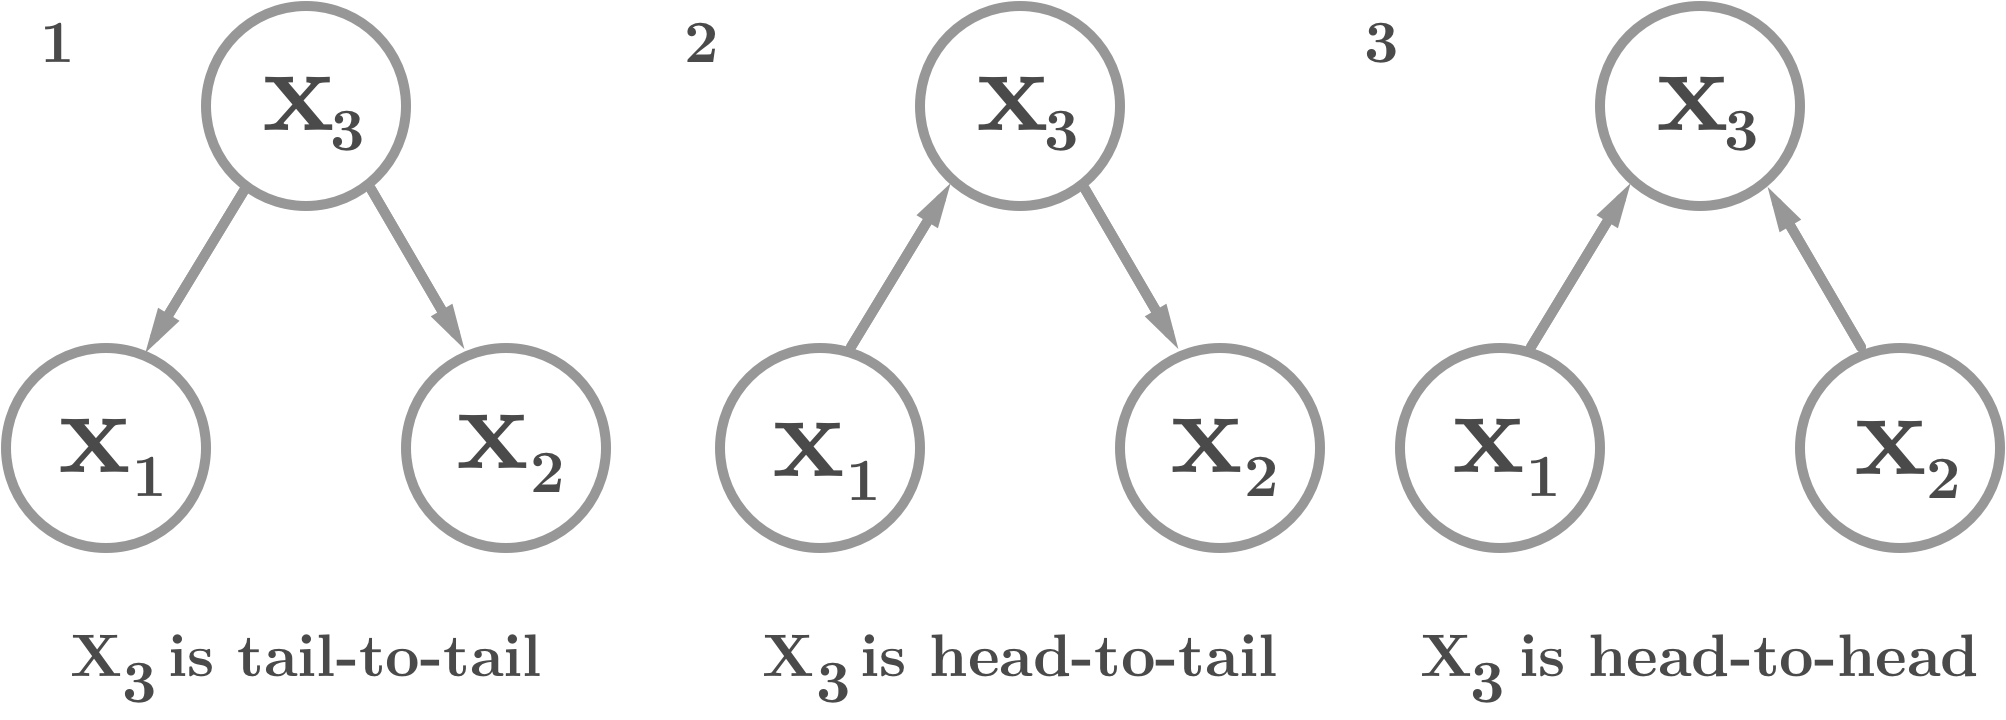
\includegraphics[width=\linewidth]{figs/bayes.png}

\begin{enumerate}
\item $p(X_1, X_2, X_3) = p(X_3)p(X_1|X_3)p(X_2|X_3)$ : $X_1$ and $X_2$ are independent given $X_3$
\item $p(X_1, X_2, X_3) = p(X_1)p(X_3|X_1)p(X_2|X_3)$ : $X_1$ and $X_2$ are independent given $X_3$
\item $p(X_1, X_2, X_3) = p(X_1)p(X_2)p(X_3|X_1, X_2)$ : $X_1$ and $X_2$ are \textbf{not} independent given $X_3$
\end{enumerate}

$X \rightarrow Y$ path blocked by $Z$ if it contains a variable such that either
\begin{enumerate}
\item variable is in $Z$ and it is head-to-tail or tail-to-tail
\item node is head-to-head and neither this node nor any of its descendants are in $Z$.
\end{enumerate}

$X$ and $Y$ are D-separated by $Z$ iff every path $X \rightarrow Y$ is blocked by $Z$.

$X$ is conditionally independent of $Y$ conditioned on the $Z$ if $X$ and $Y$ are D-separated by $Z$. Independence is symmetric.

The Markov blanket of a node $X_i$ is the set of parents, children, and co-parents of the node $X_i$ (other parents of its children).
